\section{The Fundamental Theorem of Calculus, part II} \label{S:4.4.FTC}

\begin{goals}
\item How can we find the exact value of a definite integral without taking the limit of a Riemann sum?
\item What is the statement of the Fundamental Theorem of Calculus Part II, and how do antiderivatives of functions play a key role in applying the theorem?
\item What is the meaning of the definite integral of a rate of change in contexts other than when the rate of change represents velocity?
\item What is an indefinite integral and how is its notation used in discussing antiderivatives?
\item How do the First and Second Fundamental Theorems of Calculus enable us to formally see how differentiation and integration are almost inverse processes?
\end{goals}

%------------------------------------
% SUBSECTION INTRODUCTION
%------------------------------------
\subsection*{Introduction}

\begin{marginfigure}[5in] % MARGIN FIGURE
\margingraphics{figs/4/4-5_VelF.pdf}
\caption{A velocity function.} \label{fig:4-5_VelF}
\end{marginfigure}

Much of our work in Chapter~\ref{CH:4} has been motivated by the velocity-distance problem:  if we know the instantaneous velocity function, $v(t)$, for a moving object on a given time interval $[a,b]$, can we determine its exact distance traveled on $[a,b]$?  In the vast majority of our discussion in Sections~\ref{S:4.1.VelocityDistance}-\ref{S:4.3.DefiniteIntegral}, we have focused on the fact that this distance traveled is connected to the area bounded by $y = v(t)$ and the $t$-axis on $[a,b]$.  In particular, for any nonnegative velocity function $y = v(t)$ on $[a,b]$, we know that the exact area bounded by the velocity curve and the $t$-axis on the interval tells us the total distance traveled, which is also the value of the definite integral $\int_a^b v(t) \, dt$.  In the situation where velocity is sometimes negative, the total area bounded by the velocity function still tells us distance traveled, while the net signed area that the function bounds tells us the object's change in position.  Recall, for instance, the introduction to Section~\ref{S:4.2.Riemann}, where we observed that for the velocity function in Figure~\ref{fig:4-5_VelF}, the total distance $D$ traveled by the moving object on $[a,b]$ is 
\[ D = A_1 + A_2 + A_3, \]
while the total change in the object's position on $[a,b]$ is 
\[ s(b) - s(a) = A_1 - A_2 + A_3. \]
While the areas $A_1$, $A_2$, and $A_3$, which are each given by definite integrals, may be computed through limits of Riemann sums (and in select special circumstances through familiar geometric formulas), in the present section we turn our attention to an alternate approach, similar to the one we encountered in Activity~\ref{A:4.1.2}.  To explore these ideas further, we consider the following preview activity.

\begin{pa} \label{PA:4.5}
A student with a third floor dormitory window $32$ feet off the ground tosses a water balloon straight up in the air with an initial velocity of $16$ feet per second.  It turns out that the instantaneous velocity of the water balloon is given by the velocity function $v(t) = -32t + 16$, where $v$ is measured in feet per second and $t$ is measured in seconds.
\ba
\item Let $s(t)$ represent the height of the water balloon above the ground at time $t$, and note that $s$ is an antiderivative of $v$.  That is, $v$ is the derivative of $s$: $v(t) = s'(t)$.  Find a formula for $s(t)$ that satisfies the initial condition that the balloon is tossed from $32$ feet above ground.  In other words, make your formula for $s$ satisfy $s(0) = 32$.
\item At what time does the water balloon reach its maximum height?  At what time does the water balloon land?
\item Compute the three differences $s \left( \frac{1}{2} \right) - s(0)$, $s(2) - s \left( \frac{1}{2} \right)$, and $s(2) - s(0)$.  What do these differences represent?
\item What is the total vertical distance traveled by the water balloon from the time it is tossed until the time it lands?
\item Sketch a graph of the velocity function $y = v(t)$ on the time interval $[0,2]$.  What is the total net signed area bounded by $y = v(t)$ and the $t$-axis on $[0,2]$?  Answer this question in two ways:  first by using your work above, and then by using a familiar geometric formula to compute areas of certain relevant regions.
\ea
\end{pa} 

\afterpa % PREVIEW ACTIVITY

%-------------------------------------------------------------------------------
% SUBSECTION THE FUNDAMENTAL THEOREM OF CALCULUS, PART II
%-------------------------------------------------------------------------------
\subsection*{The Fundamental Theorem of Calculus, Part II} \index{fundamental theorem of calculus}

\begin{marginfigure}[2in] % MARGIN FIGURE
\margingraphics{figs/4/4-5_VelV.pdf}
\caption{Finding the distance traveled when we know an object's velocity function $v$.} \label{fig:4-5_VelV}
\end{marginfigure}

Consider the setting where we know the position function $s(t)$ of an object moving along an axis, as well as its corresponding velocity function $v(t)$, and for the moment let us assume that $v(t)$ is positive on $[a,b]$.  Then, as shown in Figure~\ref{fig:4-5_VelV}, we know two different perspectives on the distance, $D$, the object travels: one is that $D = s(b) - s(a)$, which is the object's change in position.  The other is that the distance traveled is the area under the velocity curve, which is given by the definite integral, so $D = \int_a^b v(t) \, dt$.

Of course, since both of these expressions tell us the distance traveled, it follows that they are equal, so
\begin{equation} \label{E:FTCVel}
s(b) - s(a) = \int_a^b v(t) \, dt.
\end{equation}
Furthermore, we know that Equation~(\ref{E:FTCVel}) holds even when velocity is sometimes negative, since $s(b) - s(a)$ is the object's change in position over $[a,b]$, which is simultaneously measured by the total net signed area on $[a,b]$ given by $\int_a^b v(t) \, dt$.

Perhaps the most powerful part of Equation~(\ref{E:FTCVel}) lies in the fact that we can compute the integral's value if we can find a formula for $s$.  Remember, $s$ and $v$ are related by the fact that $v$ is the derivative of $s$, or equivalently that $s$ is an \emph{antiderivative} of $v$.  For example, if we have an object whose velocity is $v(t) = 3t^2 + 40$ feet per second (which is always nonnegative), and wish to know the distance traveled on the interval $[1,5]$, we have that
\begin{eqnarray*}
D & = & \int_1^5 v(t) \,dt \\
& = & \int_1^5 (3t^2 + 40) \, dt \\
& = & s(5) - s(1),
\end{eqnarray*}
where $s$ is an antiderivative of $v$.  We know that the derivative of $t^3$ is $3t^2$ and that the derivative of $40t$ is $40$, so it follows that if $s(t) = t^3 + 40t$, then $s$ is a function whose derivative is $v(t) = s'(t) = 3t^2 + 40$, and thus we have found an antiderivative of $v$.  Therefore,
\begin{eqnarray*}
D & = & \int_1^5 3t^2 + 40 \, dt \\
& = & s(5) - s(1) \\
& = & (5^3 + 40 \cdot 5) - (1^3 + 40\cdot 1) \\
& = & 284 \ \mbox{feet}.
\end{eqnarray*} 

\begin{marginfigure}[2in] % MARGIN FIGURE
\margingraphics{figs/4/4-5_VelC.pdf}
\caption{The exact area of the region enclosed by $v(t) = 3t^2 + 40$ on $[1,5]$.} \label{fig:4-5_VelC}
\end{marginfigure}

Note the key lesson of this example:  to find the distance traveled, we needed to compute the area under a curve, which is given by the definite integral.  But to evaluate the integral, we found an antiderivative, $s$, of the velocity function, and then computed the total change in $s$ on the interval.  In particular, observe that we have found the exact area of the region shown in Figure~\ref{fig:4-5_VelC}, and done so without a familiar formula (such as those for the area of a triangle or circle) and without directly computing the limit of a Riemann sum. As we proceed to thinking about contexts other than just velocity and position, it turns out to be advantageous to have a shorthand symbol for a function's antiderivative.  In the general setting of a continuous function $f$, we will often denote an antiderivative of $f$ by $F$, so that the relationship between $F$ and $f$ is that $F'(x) = f(x)$ for all relevant $x$.  Using the notation $V$ in place of $s$ (so that $V$ is an antiderivative of $v$) in Equation~(\ref{E:FTCVel}), we find it is equivalent to write that
\begin{equation} \label{E:FTCV} % EQUATION
V(b) - V(a) = \int_a^b v(t) \, dt.
\end{equation}
 Now, in the general setting of wanting to evaluate the definite integral $\int_a^b f(x) \, dx$ for an arbitrary continuous function $f$, we could certainly think of $f$ as representing the velocity of some moving object, and $x$ as the variable that represents time.  And again, Equations~(\ref{E:FTCVel}) and~(\ref{E:FTCV}) hold for any continuous velocity function, even when $v$ is sometimes negative.   This leads us to see that Equation~(\ref{E:FTCV}) tells us something even more important than the change in position of a moving object: it offers a shortcut route to evaluating any definite integral, provided that we can find an antiderivative of the integrand.  The second part of the Fundamental Theorem of Calculus (FTCII) \index{FTCII} summarizes these observations.
 
\concept{The Fundamental Theorem of Calculus, part II} % CONCEPT
{If $f$ is a continuous function on $[a,b]$, and $F$ is any antiderivative of $f$, then
\[ \int_a^b f(x) \ dx = F(b) - F(a). \]
} % end concept

\proof We can use the first part of the Fundamental Theorem to prove the second part.  In the first part, we showed that the integral, or area, function 
\[ A(x) = \int_a^x f(t) \ dt \quad \mbox{for} \quad a \leq x \leq b \]
is an antiderivative of the function $f$.  We have also shown by the Mean Value Theorem that if two functions have the same derivative, then they must differ by only a constant.  In other words, if both $A$ and $F$ are antiderivatives of $f$, then $\ds F(x) = A(x) + C$, where $C$ is an arbitrary constant.

Recall that $A(a) = 0$, which implies that $F(a) = A(a) + C = C$.  Notice also that $F(b) = A(b) + C$, and we have
\begin{eqnarray*}
F(b) - F(a) & = & [A(b) + C] - [A(a) + C] \\
& = & A(b) - A(a) \\
& = & A(b).
\end{eqnarray*}
And what is $A(b)$ with respect to the area function?  $\ds A(b) = \int_a^b f(t) \ dt$, which is the same as $\ds \int_a^b f(x) \ dx$. So
\begin{eqnarray*}
F(b) - F(a) & = & \int_a^b f(x) \ dx.
\end{eqnarray*}
\qed

A common alternate notation for $F(b) - F(a)$ is 
\[ F(b) - F(a) = F(x) \Big|_a^b \]
where we read the righthand side as ``the function $F$ evaluated from $a$ to $b$.''  In this notation, the FTCII says that
\[ \int_a^b f(x) \ dx = F(x) \Big|_a^b. \]

The FTCII opens the door to evaluating exactly a wide range of integrals.  In particular, if we are interested in a definite integral for which we can find an antiderivative $F$ for the integrand $f$, then we can evaluate the integral exactly.  For instance since $\frac{d}{dx}[\frac{1}{3}x^3] = x^2$, the FTCII tells us that
\begin{eqnarray*}
\int_0^1 x^2 \, dx & = & \left. \frac{1}{3} \ x^3 \right|_0^1 \\
& = & \frac{1}{3} \ (1)^3 - \frac{1}{3} \ (0)^3 \\
& = & \frac{1}{3}.
\end{eqnarray*}

\vspace*{-.25cm}

\begin{example} % EXAMPLE
We spent a great deal of time in the previous sections studying $\int_0^4(4x-x^2)\ dx$. Using the second part of the Fundamental Theorem of Calculus (FTCII), let's evaluate this definite integral.

\solution We need an antiderivative of $f(x)=4x-x^2$, or a function whose derivative is $4x - x^2$.  Such a function, and hence antiderivative of $f(x)$, would be $F(x) = 2x^2 - \frac{1}{3}x^3$.

By FTCII,
\[ \int_a^b f(x) = F(b) - F(a); \] 
therefore,
\begin{align*}
\int_0^4 \left( 4x - x^2 \right) \ dx & = F(4) - F(0) \\
& = \left. 2x^2 - \frac{1}{3}x^3 \right|_0^4 \\
& = \left( 2(4)^2-\frac{1}{3}4^3 \right) - \left( 0 - 0 \right) \\
& =  32-\frac{64}{3} = \frac{32}{3}.
\end{align*}
Notice that this is the same answer we obtained using limits in the previous sections, just with much less work.
\end{example} % EXAMPLE

\begin{example}
Suppose a ball is thrown straight up with velocity given by $v(t) = -32t+20$ ft/s, where $t$ is measured in seconds. Find, and interpret, $\ds \int_0^1 v(t) \ dt.$

\solution Using the second part of the Fundamental Theorem of Calculus, we have 
\begin{align*}
\int_0^1 v(t)\ dt &= \int_0^1 (-32t+20)\ dt \\
			&= -16t^2 + 20t\Big|_0^1 \\
			&= 4
\end{align*}
Thus if a ball is thrown straight up into the air with velocity $v(t) = -32t+20$, the height of the ball, $1$ second later, will be $4$ feet above the initial height. (Note that the ball has \textit{traveled} much farther. It has gone up to its peak and is falling down, but the difference between its height at $t=0$ and $t=1$ is $4$ feet.)
\end{example} % EXAMPLE

But finding an antiderivative can be far from simple; in fact, often finding a formula for an antiderivative is very hard or even impossible.  While we can differentiate just about any function, even some relatively simple ones don't have an elementary antiderivative.  A significant portion of integral calculus (which is the main focus of second semester college calculus) is devoted to understanding the problem of finding antiderivatives.

%---------------------------------------------
% SUBSECTION BASIC ANTIDERIVATIVES
%---------------------------------------------
\subsection*{Basic antiderivatives}

The general problem of finding an antiderivative is difficult.  In part, this is due to the fact that we are trying to undo the process of differentiating, and the undoing is much more difficult than the doing.  For example, while it is evident that an antiderivative of $f(x) = \sin(x)$ is $F(x) = -\cos(x)$ and that an antiderivative of $g(x) = x^2$ is $G(x) = \frac{1}{3} x^3$, combinations of $f$ and $g$ can be far more complicated.  Consider such functions as
\[ 5\sin(x) - 4x^2, \enskip x^2 \sin(x), \enskip \frac{\sin(x)}{x^2}, \enskip \mbox{and} \ \sin(x^2). \]
What is involved in trying to find an antiderivative for each?  From our experience with derivative rules, we know that while derivatives of sums and constant multiples of  basic functions are simple to execute, derivatives involving products, quotients, and composites of familiar functions are much more complicated.  Thus, it stands to reason that antidifferentiating products, quotients, and composites of basic functions may be even more challenging.  We defer our study of all but the most elementary antiderivatives to later in the text.

We do note that each time we have a function for which we know its derivative, we have a \emph{function-derivative pair}, which also leads us to knowing the antiderivative of a function.  For instance, since we know that 
\[ \frac{d}{dx}[-\cos(x)] = \sin(x), \]
it follows that $F(x) = -\cos(x)$ is an antiderivative of $f(x) = \sin(x)$.  It is equivalent to say that $f(x) = \sin(x)$ is the derivative of $F(x) = -\cos(x)$, and thus $F$ and $f$ together form the function-derivative pair.  Clearly, every basic derivative rule leads us to such a pair, and thus to a known antiderivative.   In Activity~\ref{A:4.5.1}, we will construct a list of most of the basic antiderivatives we know at this time.  Furthermore, those rules will enable us to antidifferentiate sums and constant multiples of basic functions.  For example, if $f(x) = 5\sin(x) - 4x^2$, note that since $-\cos(x)$ is an antiderivative of $\sin(x)$ and $\frac{1}{3}x^3$ is an antiderivative of $x^2$, it follows that 
\[ F(x) = -5\cos(x) - 4\cdot \frac{1}{3}x^3 \]
is an antiderivative of $f$, by the sum and constant multiple rules for differentiation.

\begin{margintable}[12cm] % MARGIN TABLE
\scalebox{1.25}{
\begin{tabular}{|l||c|}
   \hline 
\T Function & Antiderivative \ \B \\
\hline \hline
\T $k$, ($k$ is constant) & \ \B \\
\hline
\T $x^n$, $n \ne -1$ & \  \B \\
\hline 
\T $\frac{1}{x}$, $x > 0$ & \ \B \\ 
\hline
\T $\sin(x)$ & \ \B \\
\hline
\T $\cos(x)$ & \ \B \\
\hline
\T $\sec(x) \tan(x)$ & \ \B \\
\hline
\T $\csc(x) \cot(x)$ & \ \B \\
\hline
\T $\sec^2 (x)$ & \ \B \\
\hline
\T $\csc^2 (x)$ & \ \B \\
\hline
\T $e^x$  & \ \B \\
\hline
\T $a^x$ $(a > 1)$  & \ \B \\
\hline
\T $\frac{1}{1+x^2}$ & \ \B \\
\hline
\T $\frac{1}{\sqrt{1-x^2}}$ & \ \B \\
\hline
\end{tabular}
} % end scalebox 
\caption{Familiar basic functions and their antiderivatives.} \label{T:4.4.Act2}
\end{margintable}

\begin{activity} \label{A:4.5.1}  Use your knowledge of derivatives of basic functions to complete the table of antiderivatives.  For each entry, your task is to find a function $F$ whose derivative is the given function $f$.  When finished, use the FTCII and the results in the table to evaluate the given definite integrals.
\ba
\item $\ds \int_{-2}^2 x^3\ dx$
\item $\ds \int_0^\pi \sin x\ dx$
\item $\ds \int_0^5 e^t\ dt$
\item $\ds \int_4^9 \sqrt{u}\ du$
\item $\ds \int_1^5 2\ dx$
\item  $\ds \int_0^1 \left(x^3 - x - e^x + 2\right) \,dx$
\item  $\ds \int_0^{\pi/3} (2\sin (t) - 4\cos(t) + \sec^2(t) - \pi) \, dt$
\item  $\ds \int_0^1 (\sqrt{x}-x^2) \, dx$
\ea
\end{activity}

\begin{smallhint}
For the table, you might start by constructing a list of all the basic functions whose derivative you know.  For the three definite integrals, be sure to recall the sum and constant multiple rules, which work not only for differentiating, but also for antidifferentiating.
\end{smallhint}
\begin{bighint}
For the table, you might start by constructing a list of all the basic functions whose derivative you know.  For example, we know that $\frac{d}{dx} [\csc(x)] = -\csc(x) \cot(x).$  For the three definite integrals, be sure to recall the sum and constant multiple rules, which work not only for differentiating, but also for antidifferentiating.  Then use the FTC.
\end{bighint}
\begin{activitySolution}
\vfill \ 
\pagebreak

\begin{center}
\begin{tabular}{ | l || l | }
   \hline 
\T given function, $f(x)$ \hspace{1.25in} &  antiderivative, $F(x)$  \hspace{1.15in} \ \B \\
\hline \hline
\T $k$, ($k \ne 0$) & $kx$ \B \\
\hline
\T $x^n$, $n \ne -1$ & $\frac{1}{n+1}x^{n+1}$ \B \\
\hline 
\T $\frac{1}{x}$, $x > 0$ & $\ln(x)$ \B \\ 
\hline
\T $\sin(x)$ & $-\cos(x)$ \B \\
\hline
\T $\cos(x)$ & $\sin(x)$ \B \\
\hline
\T $\sec(x) \tan(x)$ & $\sec(x)$ \B \\
\hline
\T $\csc(x) \cot(x)$ & $-\csc(x)$ \B \\
\hline
\T $\sec^2 (x)$ & $\tan(x)$ \B \\
\hline
\T $\csc^2 (x)$ & $\cot(x)$ \B \\
\hline
\T $e^x$  & $e^x$ \B \\
\hline
\T $a^x$ $(a > 1)$  & $\frac{1}{\ln(a)} a^x$ \B \\
\hline
\T $\frac{1}{1+x^2}$ & $\arctan(x)$ \B \\
\hline
\T $\frac{1}{\sqrt{1-x^2}}$ & $\arcsin(x)$ \B \\
\hline
\end{tabular} 
\end{center}

\ba
         \item  By standard antiderivative rules and the FTC, 
         \begin{eqnarray*}
           \int_0^1 \left(x^3 - x - e^x + 2\right) \,dx & = & \left. \frac{1}{4} x^4 - \frac{1}{2}x^2 - e^x + 2x \right|_0^1 \\
           			& = &  \left(\frac{1}{4} (1)^4 - \frac{1}{2}(1)^2 - e^1 + 2(1) \right) -   \left(\frac{1}{4} (0)^4 - \frac{1}{2}(0)^2 - e^0 + 2(0) \right) \\
			& = &  \frac{1}{4} - \frac{1}{2} - e + 2 -  \left(0 - 0 - 1 + 0 \right) \\
			& = & -\frac{1}{4} - e + 3 \\
			& = & \frac{11}{4} - 3.
	\end{eqnarray*}
	\item  Calculating the needed antiderivative and applying the FTC,
	\begin{eqnarray*}
	  \int_0^{\pi/3} (2\sin (t) - 4\cos(t) + \sec^2(t) - \pi) \, dt & = & \left. \left(-2\cos(t) - 4\sin(t) + \tan(t) - \pi t \right) \right|_0^{\pi/3} \\
	  		& = & \left(-2\cos(\pi/3) - 4\sin(\pi/3) + \tan(\pi/3) - \pi (\pi/3) \right) - \\
			& \ &  \left(-2\cos(0)) - 4\sin(0) + \tan(0) - \pi (0) \right) \\
			& = & -2 \cdot \frac{1}{2} - 4 \cdot \frac{\sqrt{3}}{2} + \sqrt{3} - \frac{\pi^2}{3} - (-2 - 0 + 0 - 0) \\
			& = & 1 - \sqrt{3} - \frac{\pi^2}{3}.
	\end{eqnarray*}
	\item  Noting that $\frac{d}{dx}[\frac{2}{3} x^{3/2}] = x^{1/2}$, we find that
	\begin{eqnarray*}
	   \int_0^1 (\sqrt{x} - x^2) \, dx & = & \left. \frac{2}{3}x^{3/2} - \frac{1}{3}x^3 \right|_0^1 \\
	    				& = & \frac{2}{3} - \frac{1}{3} - (0 - 0 ) \\
					& = & \frac{1}{3}.
	\end{eqnarray*}
\ea
\end{activitySolution}
\aftera % ACTIVITY

We now revisit the fact that each function has more than one antiderivative.  Because the derivative of any constant is zero, any time we seek an arbitrary antiderivative, we may add a constant of our choice.  For instance, if we want to determine an antiderivative of $g(x) = x^2$, we know that $G(x) = \frac{1}{3}x^3$ is one such function.  But we could alternately have chosen $G(x) = \frac{1}{3}x^3 + 7$, since in this case as well, $G'(x) = x^2$.  In some contexts later on in calculus, it is important to discuss the most general antiderivative of a function.  If $g(x) = x^2$, we say that the \emph{general antiderivative} \index{antiderivative!general} or \emph{indefinite integral} of $g$ is 
\[ G(x) = \frac{1}{3}x^3 + C, \]
where $C$ represents an arbitrary real number constant.  Regardless of the formula for $g$, including $+C$ in the formula for its antiderivative $G$ results in the most general possible antiderivative.

\definition{General Antiderivatives/Indefinite Integrals} % DEFINITION
{Let a function $f(x)$ be given. A \textbf{general antiderivative} or \textbf{indefinite integral} of $f(x)$ is the infinite family of  functions 
\[ F(x) + C\]
where $C$ is an arbitrary constant such that 
\[ F'(x) = f(x).\]
}% end definition

Given a function $f$ and one of its antiderivatives $F$, we know \textit{all} antiderivatives of $f$ have the form $F(x) + C$ for some constant $C$. Using the above definition, we can say that
\[ \int f(x) \ dx = F(x) + C. \]
Let's analyze this indefinite integral notation.\index{integration!notation}

\begin{figure}[h]
\begin{center}
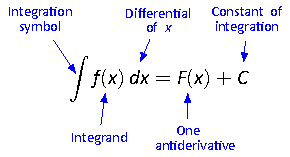
\includegraphics[scale=1.375]{figs/4/4-5_figanti1.pdf}
\caption{Understanding the indefinite integral notation.}\label{fig:4-5_figanti1}
\end{center}
\end{figure}

\begin{example}
Evaluate $\ds \int (3x^2 + 4x+5)\ dx$. 

\solution We seek a function $F(x)$ whose derivative is $3x^2+4x+5$. When taking derivatives, we can consider functions term-by-term, so we can also do that here.

What functions have a derivative of $3x^2$? Some thought will lead us to a cubic, specifically $x^3+C_1$, where $C_1$ is a constant. 

What functions have a derivative of $4x$? Here the $x$ term is raised to the first power, so we likely seek a quadratic. Some thought should lead us to $2x^2+C_2$, where $C_2$ is a constant.

Finally, what functions have a derivative of $5$? Functions of the form $5x+C_3$, where $C_3$ is a constant.

Our answer appears to be 
\[ \int (3x^2+4x+5)\ dx = x^3+C_1+2x^2+C_2+5x+C_3.\]
We do not need three separate constants of integration; combine them as one constant, giving the final answer of 
\[ \int (3x^2+4x+5)\ dx = x^3+2x^2+5x+C.\]
It is easy to verify our answer; take the derivative of $x^3+2x^3+5x+C$ and see we indeed get $3x^2+4x+5$.
\end{example} % EXAMPLE

This final step of ``verifying our answer'' is important both practically and theoretically. In general, taking derivatives is easier than finding antiderivatives so checking our work is easy and vital as we learn.  We also see that taking the derivative of our answer returns the function in the integrand. Thus we can say that: 
\[ \frac{d}{dx}\left(\int f(x)\ dx\right) = f(x). \]
Differentiation ``undoes'' the work done by antidifferentiation. 

%--------------------------------------------------
% SUBSECTION INITIAL VALUE PROBLEMS
%--------------------------------------------------
\subsection*{Initial Value Problems}

We have seen that the derivative of a position function gave a velocity function, and the derivative of a velocity function describes the acceleration.\index{initial value problem} We can now go ``the other way:'' the antiderivative of an acceleration function gives a velocity function, etc. While there is just one derivative of a given function, there are infinite antiderivatives. Therefore we cannot ask ``What is \textit{the} velocity of an object whose acceleration is $-32$ft/s$^2$?'', since there is more than one answer. 

We can find \textit{the} answer if we provide more information with the question, as done in the following example.

\begin{example}
The acceleration due to gravity of a falling object is $-32$ ft/s$^2$. At time $t=3$, a falling object had a velocity of $-10$ ft/s. Find the equation of the object's velocity.
We want to know a velocity function, $v(t)$. We know two things:
\begin{itemize}
\item The acceleration, i.e., $v'(t)= -32$, and
\item the velocity at a specific time, i.e., $v(3) = -10$.
\end{itemize}
Using the first piece of information, we know that $v(t)$ is an antiderivative of $v'(t)=-32$. So we begin by finding the indefinite integral of $-32$:
\[ \int (-32)\ dt = -32t+C=v(t). \]
Now we use the fact that $v(3)=-10$ to find $C$:
\begin{align*}
v(t) &= -32t+C \\
v(3) &= -10 \\
-32(3)+C &= -10\\
C &= 86
\end{align*}

Thus $v(t)= -32t+86$. We can use this equation to understand the motion of the object: when $t=0$, the object had a velocity of $v(0) = 86$ ft/s. Since the velocity is positive, the object was moving upward.

When did the object begin moving down? Immediately after $v(t) = 0$:
\[ -32t+86 = 0 \quad \Rightarrow \quad  t = \frac{43}{16}  \approx 2.69\text{ s}. \]
Recognize that we are able to determine quite a bit about the path of the object knowing just its acceleration and its velocity at a single point in time.
\end{example} % EXAMPLE

\begin{example}
Find $f(t)$, given that $f''(t) = \cos t$, $f'(0) = 3$ and $f(0) = 5$.
We start by finding $f'(t)$, which is an antiderivative of $f''(t)$:
\[ \int f''(t)\ dt = \int \cos t\ dt = \sin t + C = f'(t). \]
	
So $f'(t) = \sin t+C$ for the correct value of $C$. We are given that $f'(0) = 3$, so:
\[ f'(0) = 3 \quad \Rightarrow \quad \sin 0+C = 3 \quad \Rightarrow \quad C=3. \]
Using the initial value, we have found $f'(t) = \sin t+ 3.$
		
We now find $f(t)$ by integrating again.

\[ \int f'(t) \ dt = \int (\sin t+3)\ dt = -\cos t + 3t + C. \]
We are given that $f(0) = 5$, so
\begin{align*}
-\cos 0 + 3(0) + C &= 5 \\
-1 + C &= 5\\
C &= 6
\end{align*}
Thus $f(t) = -\cos t + 3t + 6$.
\end{example} % EXAMPLE

\begin{activity} \label{A:4.5.2}  Given the following velocity functions and initial positions of some objects, produce the position functions of the objects.
\ba
\item $\ds v(t) = 3t - 5; \enskip s(1) = 3$
\item $\ds v(t) = 8 \sin(t); \enskip s(\pi/6) = 8$
\item $\ds v(t) = \frac{3}{t} + 6; \enskip s(1) = 8$
\ea
\end{activity}
 % ACTIVITY

%-------------------------------------------------------------------------------------------
% SUBSECTION DIFFERENTIATING AN INTEGRAL FUNCTION
%-------------------------------------------------------------------------------------------

\subsection*{Differentiating an Integral Function}

We have seen that the Fundamental Theorem of Calculus (FTC) enables us to construct an antiderivative $F$ of any continuous function $f$ by defining $A$ by the corresponding integral function $A(x) = \int_c^x f(t) \, dt$.  Said differently, if we have a function of the form $A(x) = \int_c^x f(t) \, dt$, then we know that $A'(x) = \frac{d}{dx} \left[\int_c^x f(t) \, dt \right] = f(x)$.  This shows that integral functions, while perhaps having the most complicated formulas of any functions we have encountered, are nonetheless particularly simple to differentiate.  For instance, if 
\[ A(x) = \int_{\pi}^x \sin(t^2) \ dt, \]
then by the FTC, we know immediately that
\[ A'(x) = \sin(x^2). \]

Restating this result more generally for an arbitrary function $f$, we know by the FTC that
\[ \frac{d}{dx} \left[ \int_a^x f(t) \, dt \right] = f(x). \]
In words, the last equation essentially says that ``the derivative of the integral function whose integrand is $f$, is $f$.''  In this sense, we see that if we first integrate the function $f$ from $t = a$ to $t = x$, and then differentiate with respect to $x$, these two processes ``undo'' one another.

Taking a different approach, say we begin with a function $f(t)$ and differentiate with respect to $t$.  What happens if we follow this by integrating the result from $t = a$ to $t = x$?  That is, what can we say about the quantity
\[ \int_a^x \frac{d}{dt} \left[ f(t) \right] \, dt? \]
Here, we use the First FTC and note that $f(t)$ is an antiderivative of $\frac{d}{dt} \left[ f(t) \right].$  Applying this result and evaluating the antiderivative function, we see that
\begin{eqnarray*}
\int_a^x \frac{d}{dt} \left[ f(t) \right] \, dt & = & f(t) \bigg\vert_a^x \\
							& = & f(x) - f(a).
\end{eqnarray*} 
Thus, we see that if we apply the processes of first differentiating $f$ and then integrating the result from $a$ to $x$, we return to the function $f$, minus the constant value $f(a)$.  So in this situation, the two processes almost undo one another, up to the constant $f(a)$.

The observations made in the preceding two paragraphs demonstrate that differentiating and integrating (where we integrate from a constant up to a variable) are almost inverse processes.  In one sense, this should not be surprising:  integrating involves antidifferentiating, which reverses the process of differentiating.  On the other hand, we see that there is some subtlety involved, as integrating the derivative of a function does not quite produce the function itself.  This is connected to a key fact we observed, which is that any function has an entire family of antiderivatives, and any two of those antiderivatives differ only by a constant.

\newpage

%-------------
% SUMMARY
%-------------
\begin{summary}
\item We can find the exact value of a definite integral without taking the limit of a Riemann sum or using a familiar area formula by finding the antiderivative of the integrand, and hence applying the Fundamental Theorem of Calculus.
\item The Fundamental Theorem of Calculus says that if $f$ is a continuous function on $[a,b]$ and $F$ is an antiderivative of $f$, then
\[ \int_a^b f(x) \, dx = F(b) - F(a). \]
Hence, if we can find an antiderivative for the integrand $f$, evaluating the definite integral comes from simply computing the change in $F$ on $[a,b]$. 
\item A slightly different perspective on the FTC allows us to restate it as the Total Change Theorem, which says that
\[ \int_a^b f'(x) \, dx = f(b) - f(a), \]
for any continuously differentiable function $f$.   This means that the definite integral of the instantaneous rate of change of a function $f$ on an interval $[a,b]$ is equal to the total change in the function $f$ on $[a,b]$.
\end{summary}

\clearpage

%--------------
% EXERCISES
%--------------
\begin{adjustwidth*}{}{-2.25in}
\textbf{{\large Exercises}}
\setlength{\columnsep}{25pt}
\begin{multicols*}{2}
\noindent Terms and Concepts \small
\begin{enumerate}[1)]
\item Define the term ``antiderivative'' in your own words.
\item Is it more accurate to refer to ``the'' antiderivative of $f(x)$ or ``an'' antiderivative of $f(x)$?
\item Use your own words to define the indefinite integral of $f(x)$.
\item Fill in the blanks: ``Inverse operations do the \underline{\hskip .5in} things in the \underline{\hskip .5in} order.''
\item The derivative of a position function is a \underline{\hskip .5in} function.
\item The antiderivative of an acceleration function is a \underline{\hskip .5in} function.
\item How are definite and indefinite integrals related?
\item What constant of integration is most commonly used when evaluating definite integrals?
\item The definite integral can be used to find ``the area under a curve.'' Give two other uses for definite integrals.
\end{enumerate} 

\noindent {\normalsize Problems} \small

\noindent{\bf In exercises 4--27, evaluate the indefinite integral.}

\bmtwo
\begin{enumerate}[1),resume]
\item $\ds \int 3x^3\ dx$
\item $\ds \int x^8\ dx$
\item $\ds \int (10x^2-2)\ dx$
\item $\ds \int  dt$
\item $\ds \int 1\  ds$
\item $\ds \int \frac{1}{3t^2}\  dt$
\item $\ds \int \frac{3}{t^2}\  dt$
\item $\ds \int \frac{1}{\sqrt{x}}\  dx$
\item $\ds \int \sec^2(\theta)\  d\theta$
\item $\ds \int \sin(\theta)\  d\theta$
\item $\ds \int 5e^\theta\  d\theta$
\item $\ds \int 3^t\  dt$
\item $\ds \int \frac{5^t}{2}\  dt$
\item $\ds \int (2t+3)^2\  dt$
\item $\ds \int (t^2+3)(t^3-2t)\  dt$
\item $\ds \int x^2x^3\  dx$
\item $\ds \int e^\pi\  dx$
\item $\ds \int t\  dx$
\end{enumerate}
\emtwo

\noindent{\bf In exercises 28--38, solve the initial value problem.}

\begin{enumerate}[1),start=28]
\item $\fp(x) = \sin (x)$ and $f(0)= 2$
\item $\fp(x) = 5e^x$ and $f(0)= 10$
\item $\fp(x) = 4x^3-3x^2$ and $f(-1)= 9$
\item $\fp(x) = \sec^2 (x)$ and $f(\pi/4)= 5$
\item $\fp(x) = 7^x$ and $f(2)= 1$
\item $\fpp(x) = 5$ and $\fp(0)= 7$, $f(0) = 3$
\item $\fpp(x) = 7x$ and $\fp(1)= -1$, $f(1) = 10$
\item $\fpp(x) = 5e^x$ and $\fp(0)= 3$, $f(0) = 5$
\item $\fpp(x) = \sin (\theta)$ and $\fp(\pi)= 2$, $f(\pi) = 4$
\item $\fpp(x) = 24x^2+2^x-\cos (x)$ and $\fp(0)= 5$, $f(0) = 0$
\item $\fpp(x) = 0$ and $\fp(1)= 3$, $f(1) = 1$
\end{enumerate}

\noindent{\bf In exercises 39--51, evaluate the definite integral.}

\bmtwo
\begin{enumerate}[1),resume]
\item $\ds\int_1^3 (3x^2-2x+1)\ dx$
\item $\ds\int_0^4 (x-1)^2\ dx$
\item $\ds\int_{-1}^1 (x^3-x^5)\ dx$
\item $\ds\int_{\pi/2}^\pi \cos (x)\ dx$
\item $\ds\int_{0}^{\pi/4} \sec^2 (x)\ dx$
\item $\ds\int_{1}^{e} \frac1x \ dx$
\item $\ds\int_{-1}^{1} 5^x \ dx$
\item $\ds\int_{-2}^{-1} (4-2x^3) \ dx$
\item $\ds\int_{1}^{3} e^x \ dx$
\item $\ds\int_{0}^{4} \sqrt{t} \ dt$
\item $\ds\int_{9}^{25} \frac{1}{\sqrt{t}} \ dt$
\item $\ds\int_{1}^{8} \sqrt[3]{x} \ dx$
\item $\ds\int_{1}^{2} \frac1{x} \ dx$
\item $\ds\int_{1}^{2} \frac1{x^2} \ dx$
\item $\ds\int_{1}^{2} \frac1{x^3} \ dx$
\item $\ds\int_{0}^{1} x \ dx$
\item $\ds\int_{0}^{1} x^2 \ dx$
\item $\ds\int_{0}^{1} x^3 \ dx$
\item $\ds\int_{0}^{1} x^{100} \ dx$
\item $\ds\int_{-4}^{4} \ dx$
\item $\ds\int_{-10}^{-5} 3\ dx$
\item $\ds\int_{-2}^{2} 0\ dx$
\item $\ds \int_{\pi/6}^{\pi/3} \csc (x)\cot (x)\ dx$
\end{enumerate}
\emtwo

\begin{enumerate}[1),start=62]
\item $\ds\int_{0}^{\pi} (2\cos (x) - 2\sin (x)) \ dx$
\item Explain why:
\begin{enumerate}
\item		$\ds \int_{-1}^1 x^n\ dx=0$, when $n$ is a positive, odd integer, and 
\item		$\ds \int_{-1}^1 x^n\ dx = 2\int_{0}^1 x^n\ dx$ when $n$ is a positive, even integer.
\end{enumerate}
\end{enumerate}

\noindent{\bf In exercises 64--68, a velocity function of an object moving along a straight line is given. Find the displacement of the object over the given time interval.}

\begin{enumerate}[1),resume]
\item $v(t) = -32t+20$ ft/s on $[0,5]$
\item $v(t) = -32t+200$ ft/s on $[0,10]$
\item $v(t) = 2^t$ mph on $[-1,1]$
\item $v(t) = \cos (t)$ ft/s on $[0,3\pi/2]$
\item $v(t) = \sqrt[4]{t}$ ft/s on $[0,16]$
\end{enumerate}

%------------------------------------------
% END OF EXERCISES ON FIRST PAGE
%------------------------------------------
\end{multicols*}
\end{adjustwidth*}

\clearpage

\begin{adjustwidth*}{}{-2.25in}
\setlength{\columnsep}{25pt}
\begin{multicols*}{2}\small

\noindent{\bf In Exercises 69--72, an acceleration function of an object moving along a straight line is given. Find the change of the object's velocity over the given time interval.}

\begin{enumerate}[1),start=69]
\item $a(t) = -32$ ft/s$^2$ on $[0,2]$
\item $a(t) = 10$ ft/s$^2$ on $[0,5]$
\item $a(t) = t$ ft/s$^2$ on $[0,2]$
\item $a(t) = \cos (t)$ ft/s$^2$ on $[0,\pi]$

    \item A function $f$ is given piecewise by the formula
  $$f(x) = \left\{ 
  	\begin{array}{lr}
	-x^2 + 2x + 1, & \ \mbox{if} \ 0 \le x < 2 \\
	-x + 3, & \ \mbox{if} \ 2 \le x < 3 \\
	x^2 - 8x + 15, & \ \mbox{if} \ 3 \le x \le 5
	\end{array}
	\right.
  $$
  \ba
  	\item Determine the exact value of the net signed area enclosed by $f$ and the $x$-axis on the interval $[2,5]$.
	\item Compute the exact average value of $f$ on $[0,5]$.
	\item Find a formula for a function $g$ on $5 \le x \le 7$ so that if we extend the above definition of $f$ so that $f(x) = g(x)$ if $5 \le x \le 7$, it follows that $\int_0^7 f(x) \, dx = 0.$
  \ea
\end{enumerate}

\begin{enumerate}[1),resume]
 \item The instantaneous velocity (in meters per minute) of a moving object is given by the function $v$ as pictured below.  Assume that on the interval $0 \le t \le 4$, $v(t)$ is given by $v(t) = -\frac{1}{4}t^3 + \frac{3}{2}t^2 + 1$, and that on every other interval $v$ is piecewise linear, as shown.

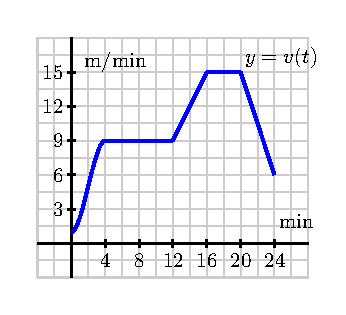
\includegraphics[scale=.75]{figures/4_4_Ez2.eps}

    \ba
  	\item Determine the exact distance traveled by the object on the time interval $0 \le t \le 4$.
	\item What is the object's average velocity on $[12,24]$?
	\item At what time is the object's acceleration greatest?
	\item Suppose that the velocity of the object is increased by a constant value $c$ for all values of $t$.  What value of $c$ will make the object's total distance traveled on $[12,24]$ be $210$ meters?
  \ea
  
    \item When an aircraft attempts to climb as rapidly as
possible, its climb rate (in feet per minute) decreases as altitude
increases, because the air is less dense at higher altitudes.
Given below is a table showing performance data for a certain
single engine aircraft, giving its climb rate at various altitudes, where  $c(h)$ denotes the climb rate of the airplane at an altitude $h$.


\begin{center}
\scalebox{.85}{
  \begin{tabular}{|c||c|c|c|c|c|c|}
    \hline
    $h$ (feet)& $0$ & $1000$ & $2000$ & $3000$ & $4000$ & $5000$\\
    \hline
    $c$ (ft/min)& $925$ & $875$ & $830$ & $780$ & $730$ & $685$\\
    \hline
    \hline
    $h$ (feet)& $6000$ & $7000$ & $8000$ & $9000$ & $10,000$ &\\
    \hline
    $c$ (ft/min)& $635$ & $585$ & $535$ & $490$ & $440$ &\\
    \hline
  \end{tabular}
  }
\end{center}


 Let a new function called $m(h)$ measure
the number of minutes required for a plane at altitude $h$ to climb the
next foot of altitude.
\ba
	\item Determine a similar table of values for $m(h)$ and explain how it is related to the table above.  Be sure to explain the units.

	\item Give a careful interpretation of a function whose derivative
is $m(h)$.  Describe what the input is and what the output is.  Also,
explain in plain English what the function tells us.

	\item Determine a definite integral whose value tells us exactly the number of minutes required for the airplane to ascend to
$10,000$ feet of altitude.  Clearly explain why the value of this integral has the required meaning.

	\item Use the Riemann sum $M_5$ to estimate the value of the integral you found in (c).  Include units on your result.
\ea


\end{enumerate}

%---------------------------------------------
% END OF EXERCISES ON SECOND PAGE
%---------------------------------------------
\end{multicols*}
\end{adjustwidth*}

\afterexercises 

\cleardoublepage